\hypertarget{a00349}{}\section{Parameter automation}
\label{a00349}\index{Parameter automation@{Parameter automation}}
Information about parameter automation. 

\hypertarget{a00349_parameterAutomation_contents}{}\subsection{On this page}\label{a00349_parameterAutomation_contents}
 \hypertarget{a00349_parameterAutomation_overview}{}\subsection{Overview}\label{a00349_parameterAutomation_overview}
 The term \char`\"{}automation\char`\"{} can mean two things in A\+A\+X\+: 
\begin{DoxyEnumerate}
\item A host feature allowing users to record and play back plug-\/in parameter changes. In this documentation, this data is referred to as {\itshape {\bfseries automation data}}, and it is stored in {\itshape {\bfseries automation lanes}} in the host.  
\item A system for arbitrating between changes from different parameter editors such as the plug-\/in G\+U\+I, control surfaces, and pre-\/recorded automation values. In this documentation, this is referred to as the {\itshape {\bfseries event system}} for parameters.  
\end{DoxyEnumerate}

 Here are some examples of how these two different meanings are used in A\+A\+X\+: \begin{DoxyItemize}
\item The \hyperlink{a00086}{A\+A\+X\+\_\+\+I\+Automation\+Delegate} provides methods for interacting with the host\textquotesingle{}s parameter event system. \item \hyperlink{a00061_a4e6eeef25a797ea4c6961df45174b169}{A\+A\+X\+\_\+\+I\+A\+C\+F\+Effect\+Parameters\+::\+Get\+Parameter\+Is\+Automatable()} and the {\ttfamily automatable} parameter in the \hyperlink{a00033}{A\+A\+X\+\_\+\+C\+Parameter} constructor reflect whether a parameter can have automation written and read by the host. \item \hyperlink{a00090_af9ab9b228023e116f89249a56c27a20f}{A\+A\+X\+\_\+\+I\+Controller\+::\+Get\+Current\+Automation\+Timestamp()} gets the timestamp for pre-\/recorded automation data when it is received by the plug-\/in during playback\end{DoxyItemize}
For more information about the parameter event system, see the \hyperlink{a00350}{Parameter updates} pages, and particularly the information on the \hyperlink{a00352}{Token protocol} 

 \hypertarget{a00349_parameterAutomation_elements}{}\subsection{Plug-\/in elements used for automation}\label{a00349_parameterAutomation_elements}
 
\begin{DoxyImage}
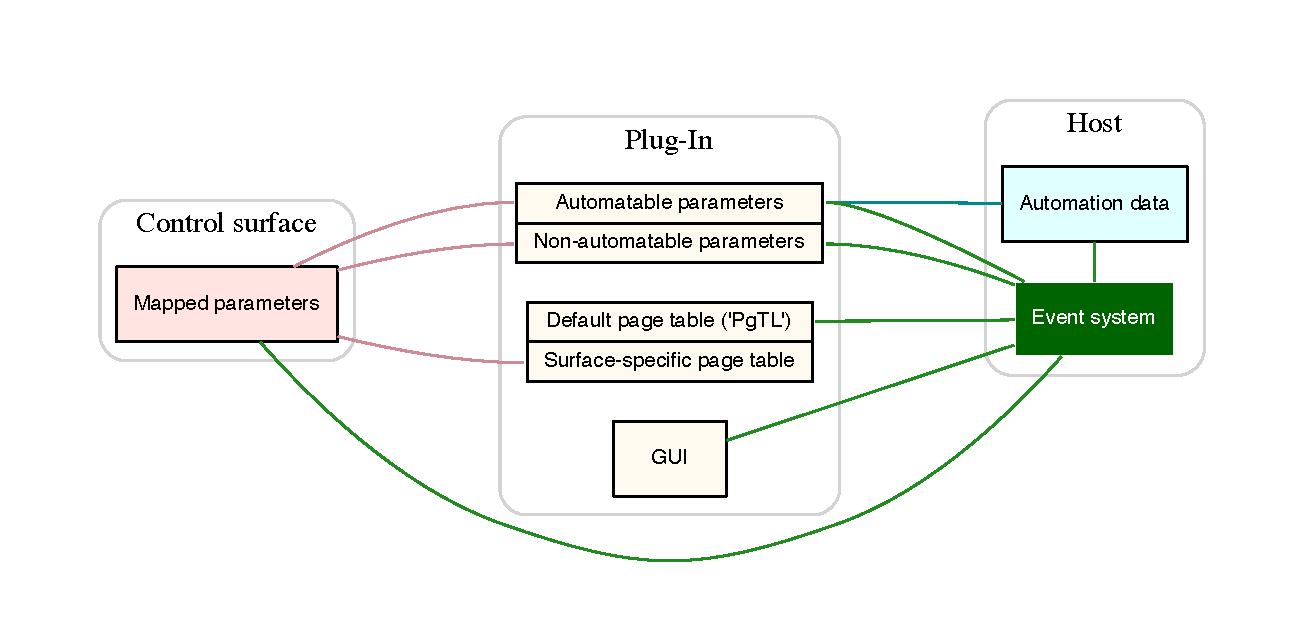
\includegraphics[width=\textwidth,height=\textheight/2,keepaspectratio=true]{dot_aax_automation_components}
\caption{Plug-\/in elements used for events and automation}
\end{DoxyImage}
 \hypertarget{a00349_parameterAutomation_definingParameters}{}\subsubsection{Defining automatable parameters}\label{a00349_parameterAutomation_definingParameters}
 In order for a parameter to be available for automation recording, editing, and playback, the plug-\/in must meet the following criteria\+: \begin{DoxyItemize}
\item It must provide {\ttfamily true} when the host calls \hyperlink{a00061_a4e6eeef25a797ea4c6961df45174b169}{Get\+Parameter\+Is\+Automatable()} for the parameter. In nearly all plug-\/ins, this means providing {\ttfamily true} to the {\ttfamily automatable} parameter in the parameter\textquotesingle{}s \hyperlink{a00033}{A\+A\+X\+\_\+\+C\+Parameter} constructor. \item It must expose the parameter to the parameter event system (see below.)\end{DoxyItemize}
In order for a parameter to be exposed to the event system, the plug-\/in must meet the following criteria\+: \begin{DoxyItemize}
\item It must respond to all parameter methods in the \hyperlink{a00099}{A\+A\+X\+\_\+\+I\+Effect\+Parameters} interface, particularly \hyperlink{a00061_a8af398b1e308849464aee5a6713a3965}{Get\+Number\+Of\+Parameters()} and \hyperlink{a00061_a5387b83e0f684a5bf0e09b24cae257d9}{Get\+Parameter\+I\+D\+From\+Index()}. Generally this is accomplished by adding an \hyperlink{a00033}{A\+A\+X\+\_\+\+C\+Parameter} object for each parameter to the plug-\/in\textquotesingle{}s \hyperlink{a00344}{Parameter Manager}. \item It must include the parameter in its one-\/parameter-\/per-\/page {\ttfamily \textquotesingle{}Pg\+T\+L\textquotesingle{}} (default) page tables. See \hyperlink{a00363_aax_page_table_guide_05_implementing_page_tables}{Implementing Page Tables} in the \hyperlink{a00363}{Page Table Guide} for more information about defining this page table type.\end{DoxyItemize}
All plug-\/in parameters must be registered with the host\textquotesingle{}s event system in order for editors, including the plug-\/in\textquotesingle{}s G\+U\+I, to work properly. Therefore a plug-\/in should always define a complete {\ttfamily \textquotesingle{}Pg\+T\+L\textquotesingle{}} (default) page table including all of its parameters, even the parameters that are not \char`\"{}automatable\char`\"{}.



 \hypertarget{a00349_parameterAutomation_advanced}{}\subsection{Advanced automation topics}\label{a00349_parameterAutomation_advanced}
 \begin{DoxyItemize}
\item \hyperlink{a00354}{Linked parameters}\end{DoxyItemize}
 Collaboration diagram for Parameter automation\+:
\nopagebreak
\begin{figure}[H]
\begin{center}
\leavevmode
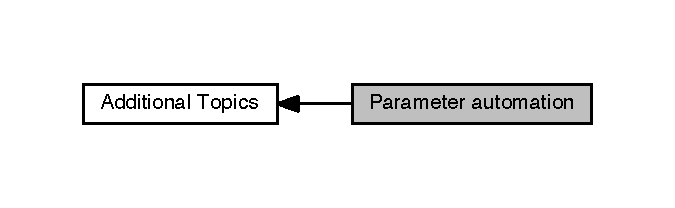
\includegraphics[width=324pt]{a00349}
\end{center}
\end{figure}
